\chapter{Background}
\label{chp:background}

This chapter provides necessary background for this dissertation, including the document classification task, methods of domain adaptation, problem settings of language variations.
This chapter organizes sections as follows:

Section~\ref{chap2:sec:doc_clf} presents a standard pipeline of building document classification models.
I first present steps of document preprocessing and major classification models. 
The classification models cover both non-neural and neural classification models, including recent advances of transformer-style models for NLP. 
I discuss methods of extracting document representations and standard evaluation metrics for document classifiers. 

Section~\ref{chap2:sec:domain_adpt} introduces important methods and frameworks for the domain adaptation, including feature augmentation, multitask learning and domain adversary learning. 
The fundamental methods serve as stepstones for new models that will be proposed in this thesis, which augment the feature representations with language variations across time and user factors and explore the benefits of joint modelings.

Section~\ref{chap2:sec:time} and Section~\ref{chap2:sec:demographic} demonstrate the challenges of handling language variations across both time and demographic factors, which can cause severe performance drops for the document classification task.
For the temporality, I discuss existing methods that model the temporal factor into neural representations, the diachronic word embedding. 
For the user factor, I present existing methods that model both user factors and potential fairness issues of document classifiers caused by user factors. 
The discussions of the language variations and existing methods serve to facilitate introductions of our proposed adaptation methods on both temporal and user factors.


\section{Document Classification}
\label{chap2:sec:doc_clf}

The task of document classification aims to assign a document one or more categories by texts, images or its associated metadata such as author information and timestamp.
This section focuses on text classification, which models classify text documents into different classes.


\subsection{Preprocessing}
Preprocessing matters for training machine learning models~\cite{camacho2018role,huang2019matters}.
Many tools can help preprocess text documents, such as NLTK~\cite{bird2004nltk}.
The process can have two different levels: text documents and document classes.
Common document preprocessing strategies include lowercase, tokenization, removing stopwords, lemmatization, etc.
For the languages like Chinese, we can use segmentation tools~\cite{sun2012jieba} to split a sentence into words.
While most of tasks focus on monolingual settings which train and test models on same languages, for the cross-lingual settings, translation is an important strategy.
Additionally, the preprocessing step is important for privacy, anonymity and fairness. 
For example for Twitter data, to protect user privacy, we can replace user name, URL and sensitive words by dummy words. Research show that replacing sensitive words in the preprocess step can significantly reduce the bias of classifiers~\cite{dixon2018measuring}.
To encode the $N$ document labels, we either choose to use sparse categorical classes such as [0, 1, ..., N-1] or one hot encoding which has one 1 and the other N-1 scalars as zeros in a numerical vector. 


\subsection{Traditional Classifiers}

Traditional classifiers including logistic regression and support vector machine (SVM) require extensive labors in designing feature sets.
In this thesis, we mainly use three types of document features: n-gram, topic model, syntax.

\begin{enumerate}
\item \textit{N-gram} approach extracts token sequences, counts their occurrence. The token sequences have different combinations of lengths, such as unigram, bi-gram or tri-gram. The count values can be normalized via tf-idf.  
\item \textit{Topic model}~\cite{blei2003latent} views each document has a distribution over $k$ topics and drive the topic features from each document. The topic feature size is the number of topics, $k$. 
\item \textit{Syntax} can be phonological, morphological, or semantic features. For example, a common feature is a part-of-speech (POS) tag, which counts number of each tag category in every document. 
\end{enumerate}  


The classifier can be trained by the input feature, x, and its associated annotations, y. Feature is a D-dimensional vector of numbers to describe the properties of an object, such as length of sentence. The annotations, or labels, are usually vectorized to  a categorical or nominal variable from some finite set, $y_i \in {1,...,C}$, where $C$ is the number of document classes. We use the features and labels to train a document classifier, $\hat{y}_i = \theta(X_i)$, by maximizing the log probability, $argmax_{\theta}\sum_{i=1}^nlog P(y_i | x_i; \theta)$, where the $i$ the index of data instance, the $\hat{y}_i$ is the predicted value by the classifier, the $\theta$ refers to the classification function. The training process is that we feed training data, x, to the classifier $\theta$ to learn the optimum values $w$. Through the model, we can predict the most probably category of the input data.


\subsection{Neural Classifiers}

Neural classifiers have shown its premier performance over traditional classifiers in document classification.
This section first introduces neural representations of words, word embedding, including embedding training process and two levels of embedding models.
Then it presents three types neural models: convolutional neural network (CNN), recurrent neural network (RNN) and bidirectional encoder representations from transformer (BERT).

\subsubsection{Word Embedding}
\label{chap2:subsubsec:emb}

\begin{figure}[t!]
\centering
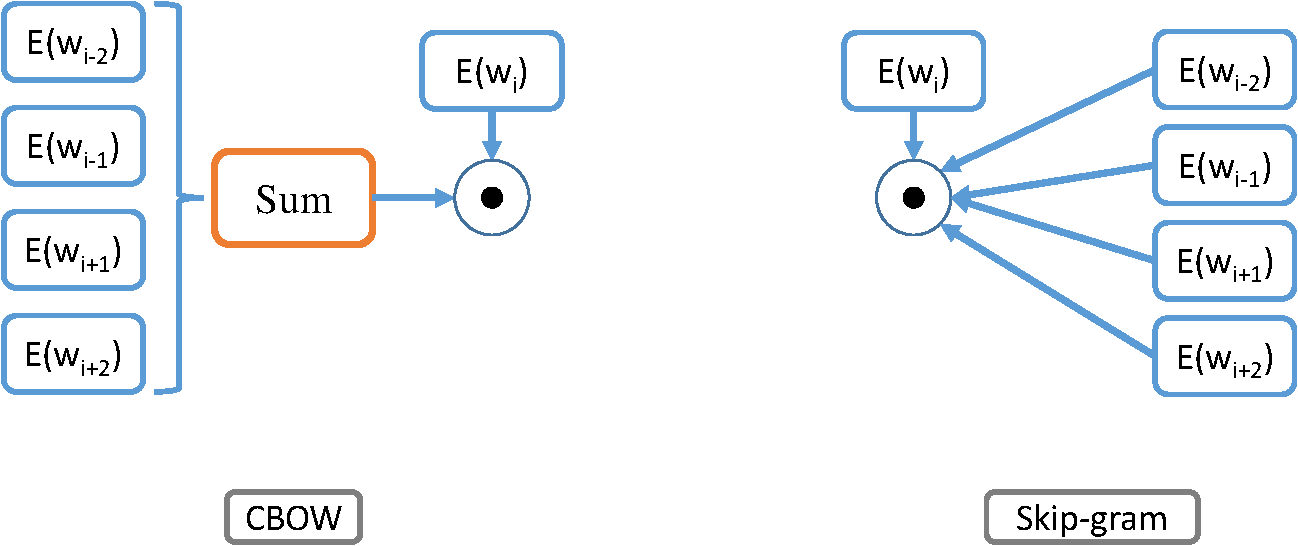
\includegraphics[width=0.55\textwidth]{images/chapter2/word2vec.pdf}
\caption{Two strategies to train word embeddings: CBOW and Skip-gram. Both methods are simple neural models with two layers: hidden layer and output layer. We use the circle to represent dot production.}
\label{chap2:fig:embd}
\end{figure}

Word embedding is to map a word into a fixed length vector. 
In this section, we will cover methods of building word embeddings from two levels, word and subword. 
We will use them extensively in the following chapters and leave out other methods that are not used in this thesis, such as character embeddings~\cite{zhang2015character}.

\paragraph{Word level} is to encode a word into a fixed dimensional representation~\cite{mikolov2013distributed, pennington2014glove}. 
There are two ways to train word embedding models, Skip-gram and Continuous Bag of Words (CBOW).
We show the details of two training strategies in Figure~\ref{chap2:fig:embd}.

The two methods both first randomly initialize the two embeddings, input ($W$) and output ($U$), with the same size $|V| * d$, where $|V|$ is the size of total vocabulary and $d$ is the vector dimension.
For the CBOW, we first generate one hot encoding vector of the context words with the context windows size as $m$ and feed the vector to the input embedding $W$; we can then obtain vector representations of the context words, $W(w_{i-m}), ..., W(w_{i-1}), W(w_{i+1}), ..., W(w_{i+m})$; next, we sum and average the obtained vectors and can get $\hat{w}$; we dot product the $\hat{w}$ with $U$ ($\theta = \hat{w} \cdot U $) and feed the output $\theta$ to a softmax function; we can obtain a predicted probability vector $\hat{y} = softmax(\theta)$ over the whole vocabulary $\hat{y} \in R^{|V|}$, and finally we can optimize the model by categorical cross-entropy $H(\hat{y}, y) = -\sum^{|V|}_{i=1}y_ilog(\hat{y}_i)$.
The key difference between the two methods is that while CBOW uses the context to predict a word, the Skip-gram predicts the context by a word.\footnote{Details of comparison can be referred to \url{https://cs224d.stanford.edu/lecture_notes/notes1.pdf}}

However, the softmax and the objective function over the whole vocabulary $V$ consume too much computation, and therefore, we use the \textit{Negative Sampling}~\cite{mikolov2013distributed} to approximate the results and reduce the computational cost.
The negative sampling use one target word and samples $n$ words as negative samples by normalized word frequency $freq^{\frac{3}{4}}$.
By only sampling some words $n \ll |V|$, the negative sampling reduces the computational cost significantly.

% draw the process of skipgram and cbow
% https://tensorflowkorea.files.wordpress.com/2017/03/cs224n-2017winter-notes-all.pdf

\paragraph{Subword level} represents a word by a couple of subwords, which are a sequence of character(s).
The method first splits a word into a series of subwords, for example, to represent $where$ by 3-gram characters, we will obtain $whe, her, ere$.
The FastText~\cite{bojanowski2017enriching} appends two positional marks, $<$ and $>$, to the start and end of each word and uses a range of n-gram characters to represent a word. 
Instead of generating a vector for a word, the method initializes an embedding for all subword components.
To represent a word, the method first sums and then averages representations of all the subword representations.
Then the model trains the aggregated word representations to either skip-gram or CBOW.
The training steps are similar to the word level embedding models shown in Figure~\ref{chap2:fig:embd}.


\subsubsection{CNN}

% draw picture and then explain in equations
\begin{figure}[htp]
\centering
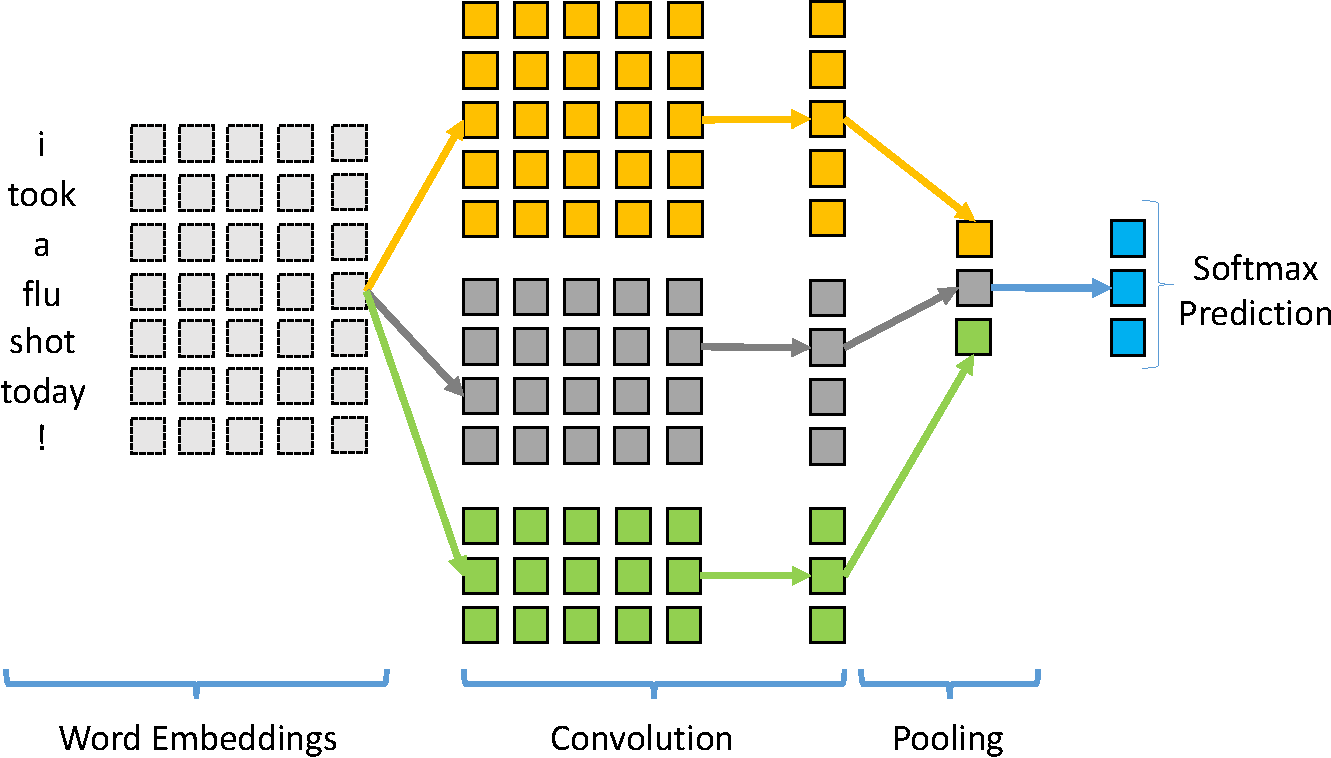
\includegraphics[width=0.55\textwidth]{images/chapter2/cnn.pdf}
\caption{Illustration of CNN model architecture for document classifiers. The simplified architecture follows the existing research work~\cite{kim2014convolutional}. We feed the indices of words to the model. The model initializes pre-trained word embeddings and deploys three different kernel sizes: 2 (yellow), 3 (grey) and 5 (green). We only use 1 filter in each kernel size for simplicity. The model perform 1-max pooling operation on the output of convolution layer. The final softmax layer receives the concatenated outputs from the pooling layer and predicts document categories.}
\label{chap2:fig:cnn}
\end{figure}

Convolutional Neural Network (CNN) has been proven its efficiency in document classification~\cite{kim2014convolutional}. 
With the example in Figure~\ref{chap2:fig:cnn}, we will introduce the basic principles of CNN document classifiers.
The model first converts a tokenized document to a vector of word indices and pad or remove the vector to a fixed length $n$. 
Then it maps the indices to a lookup table initialized by a pre-trained word embedding, such as word2vec~\cite{mikolov2013distributed}, GloVe~\cite{pennington2014glove} or FastText~\cite{bojanowski2017enriching} and then obtain a $n*d$ size of document representations.
The model then can apply 1D convolution on the document representations $A$ with zero-padding.
The convolution operation can have multiple filters with different kernel sizes $h$.
Each filter can output multiple screenshots, where each screenshot is a sub matrix of $A$, $A[i: i+h] \in R^{h*d}$ and the number of screenshot is $n-h+1$.
Therefore, we can represent the output of a screenshot as $o_i = \sigma(w \cdot A[i:i+h]) + b$, where $i \in [1, n-h+1]$, $\sigma$ is an activation function and $b$ is a bias term.
Multiple screenshots can represent generated features of a filter and feed to the pooling layer.
Besides the global max pooling method shown in Figure~\ref{chap2:fig:cnn}, we also have other pooling methods such as average pooling methods.
Finally, the classifier applies flatten operation and feed the vector to softmax function for predictions.

While CNN enjoys its parallel processing ability, it only focuses on a limited context and can not retain the long sequential information like the Recurrent Neural Network (RNN)~\cite{goodfellow2016deep}. Next section, I will briefly introduce RNN classifiers.


\subsubsection{RNN}

\begin{figure}[htp]
\centering
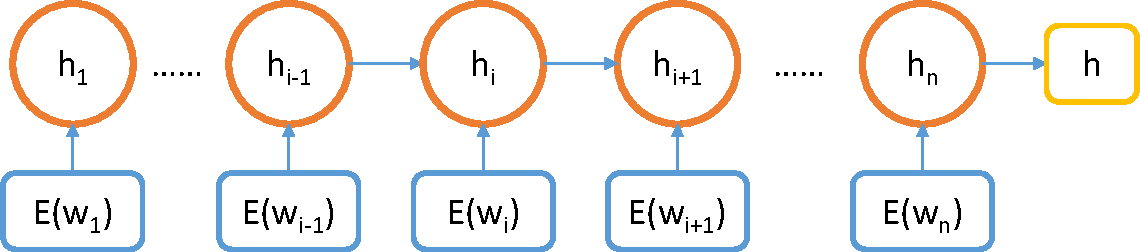
\includegraphics[width=0.55\textwidth]{images/chapter2/rnn.pdf}
\caption{Illustration of RNN model architecture for document classifiers. The RNN model reads a word in each step and recalculates its hidden state by combining the current word and the previous hidden state. The model can have one prediction per step or output its final hidden state.}
\label{chap2:fig:rnn}
\end{figure}

A key advantage of Recurrent Neural Network (RNN) is the ability of memorizing long dependency sequential information. 
We present a simple RNN model in Figure~\ref{chap2:fig:rnn}.
The model reads the current word $w_t$ every step $t$ and calculate its current hidden state $h_t$ by $h_t = f(h_{t-1}, w_t; W)$, where the $W$ is the weight of the function $f$.
We can feed the output $h$ to a softmax function for document predictions.

However, the simple RNN can suffer gradients vanish or explode and hardly capture long dependencies in practice~\cite{pascanu2013difficulty}.
We will introduce two main RNN variants, Long Term Short Memory (LSTM)~\cite{hochreiter1997long} and Gated Recurrent Unit (GRU)~\cite{chung2014empirical}.

\paragraph{LSTM} is an variation of RNN unit~\cite{hochreiter1997long} and retain more previous information by using structures called \textit{gates}.
The first gate is ``forget gate'' aiming to decide how much information we will throw away from the previous hidden state by:
$$f_t = \theta(W_f \cdot [h_{t-1}, w_t] + b_f)$$
, where $\theta$ is sigmoid function,\footnote{$\theta(x) = \frac{e^x}{e^x+1}$} $W_f$ is the weight and $b_f$ is the bias term.
The second gate is ``input gate'' aiming to decide how much information we will use to update the current memory by:
$$i_t = \theta(W_i \cdot [h_{t-1}, w_t] + b_i)$$
, where $W_i$ and $b_i$ are the weight and bias term respectively.
Before applying the input gate, we have to calculate the candidate memory value $\title{C}_t$ by $$\title{C}_t = tanh(W_c \cdot [h_{t-1}, w_t] + b_c)$$.
Now, it is time to generate the current memory by using both forget and input gates:
$$C_t = f_t * C_{t-1} + i_t * \title{C}_t$$, which is a weighted combination of previous and new information.
To obtain the output of the current cell, we compute the third gate, ``output gate'' by:
$$o_t = \theta(W_o \cdot [h_{t-1}, w_t], b_t)$$.
Finally, we can output the hidden state by:
$$h_t = o_t * tanh(C_t)$$.
We can view the output hidden state as a document representation and build a final prediction layer upon the representation.



\paragraph{GRU} is a simplified version of LSTM in two aspects: fewer gates and no memory cell~\cite{chung2014empirical}.
First, it combines the forget and input gates into one gate, ``update gate'' by:
$$z_t = \theta(W_z \cdot [h_{t-1}, w_t] + b_z)$$
, where $\theta$ is a sigmoid function, $W$ is the function weight, $h_{t-1}$ is the previous hidden state, $w_t$ is the current input information and $b$ is the bias term.
Next the GRU merges the cell memory and hidden state into one hidden state by:
$$h_t = (1-z_t) * h_{t-1} + z_t * \tilde{h}_t$$
, where $\tilde{h}_t = tanh(W_h \cdot [r_t * h_{t-1}, w_t])$.
The $r_t$ refers to a ``reset gate'' and calculates the gate by $r_t = \theta(W_r \cdot [h_{t-1}, w_t])$.
The reset gate decides to retain how much previous information.
Existing empirical research finds that the GRU shows a similar performance with the LSTM while reduces computational costs because of its simplified architecture~\cite{chung2014empirical}.


\subsubsection{BERT} 
Bidirectional Encoder Representations from Transformer (BERT)~\cite{devlin2019bert} is a Transformer~\cite{vaswani2017attention} style language model learning rich semantic information on large unlabeled corpora.
The model has two primary bases, 12 and 24 layers, which contains 110M and 340M parameters respectively.
Outputs of the model can be feature representations of documents, and we can then feed the representations to different downstream tasks.
The pre-trained model has been widely applied in several downstream tasks, such as sentiment analysis, question answering etc.

% how it pretrained: pretraining tasks
The language model learns semantic information from two unsupervised pre-training tasks: masked language modeling (Masked LM) and next sentence prediction (NSP). 
To encode a token, the BERT represents each token from three aspects: word (token), segment and position embeddings.
The word embedding is similar to the Section~\ref{chap2:subsubsec:emb}, the segment embedding indicates a token belongs to the first input segmentation or the second one, and the position embedding encodes sequential information of tokens.
For the Masked LM, the model randomly replaced 15\% of tokens in a document by a special token [MASK] and then use the encoded token representations to predict the masked tokens.
For the NSP, the model is to predict a binary relationship between two sentences that whether the second sentence actually follows the first sentence.


\subsection{Performance Evaluation}
\label{chap2:subsec:eval}

\begin{figure}[t!]
\centering
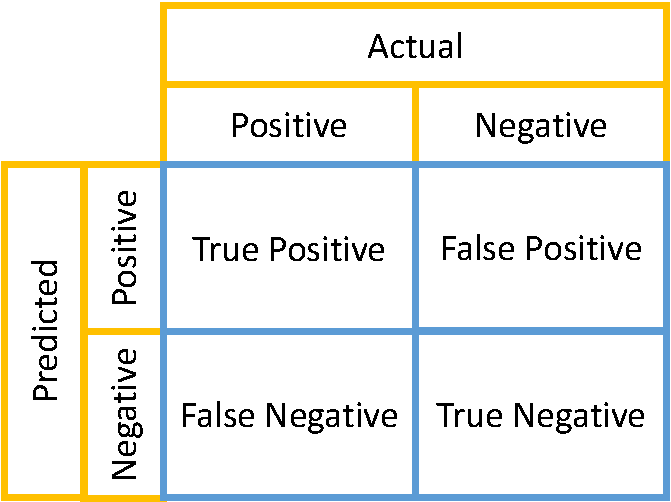
\includegraphics[width=0.55\textwidth]{images/chapter2/confusion-table.pdf}
\caption{Illustration of confusion table that summarizes prediction results of document classifiers. For simplicity, we only present classification results for binary categories. We summarize the numbers of correct and incorrect predictions with count values and broken down by each class.}
\label{chap2:fig:confusion}
\end{figure}


This section will briefly cover five evaluation metrics of the document classification task in this thesis: accuracy, precision, recall, F1-score and area under the roc curve (AUC).
The higher those metrics are, the better document classifiers are, and vice versa.
We can derive scores of the five metrics by the confusion matrix table (Figure~\ref{chap2:fig:confusion}). 
The true positive (TP), false positive (FP), false negative (FN) and true negative (TN) indicate actual and predicted values are both positive, the predicted value is true while the actual value is false, the predicted value is negative while the actual value is positive, and both of predicted and actual values are negative respectively.
The confusion matrix table can tell us insights of classification performance that what types of errors are for document classifiers.


\paragraph{Accuracy} measures correct rate of classifiers. We can calculate the accuracy score by $\frac{TP+TN}{TP+TN+FP+FN}$. Yet, the accuracy is not a good fit for imbalanced dataset. For example, if spam emails only account for 1\%, a 99\% accuracy score of a classifier is less meaningful.

\paragraph{Precision, Recall and F1-score} usually jointly measure the performance of document classification. The metrics calculate the precision by $\frac{TP}{TP+FP}$, recall by $\frac{TP}{TP+FN}$ and F1-score by $2*\frac{Recall*Precision}{Recall+Precision}$.\footnote{The F1-score derives from F-$\beta$, where F-$\beta$=$\frac{(1+\beta^2)*Precision*Recall}{(\beta^2*Precision)+Recall}$. The $\beta$ is a weight factor to balance importance of the precision and recall: the higher $\beta$ weighs recall higher than precision, and vice versa. F1-score is when the F-$\beta$ treats recall and precision equally and takes $\beta$ as 1.}
Precision measures the rate of correctly predicted instances, Recall indicates the rate of correctly recognized positive instances, and F1-score harmonically combines the precision and recall.
Yet, class labels may have skewed distributions or different weights, particularly for multi-class classification evaluation, therefore, we can average F1-scores for individual labels differently via various modes: binary, micro, macro, weighted and samples.\footnote{The modes can be referred to \url{https://scikit-learn.org/stable/modules/generated/sklearn.metrics.f1_score.html}.}


\begin{figure}[tb!]
\centering
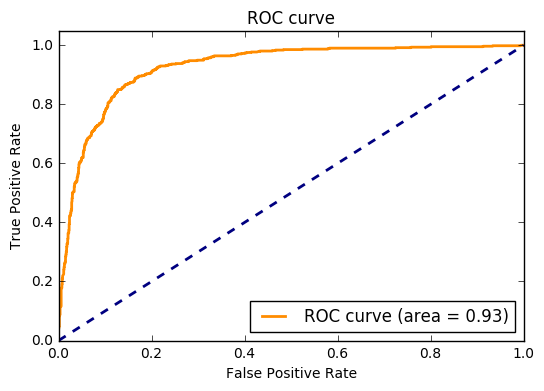
\includegraphics[width=0.55\textwidth]{images/chapter2/roc-curve.png}
\caption{Illustration of ROC curve and AUC. The AUC score can be calculated by the ROC curve, where the curves changes with classification thresholds, the X-axis indicates the FP rate and the Y-axis refers to the TP rate.}
\label{chap2:fig:roc}
\end{figure}

\paragraph{AUC} indicates how well the probabilities from the positive classes are separated from the negative classes. 
We can calculate the scores by \textit{roc\_auc\_score} function from Scikit-Learn~\cite{pedregosa2011scikit}.
Unlike the previous metrics depend on the probability threshold,\footnote{Usually we choose 0.5 as the threshold.} the AUC is classification-threshold-invariant.


% \section{Metadata and Language Variations}


\section{Domain Adaptation}
\label{chap2:sec:domain_adpt}
% domain adaptation definition;
% an illustration of domain adaptation in document classification;
% introduce what we will cover in this section
With sharing the same labels in both source and target domains, the domain adaptation aims to align source with target domain distributions so that the model trained on labeled dataset from source domain can be applied in target domain.
In this section, I will present several domain adaptation methods that will be used extensively in this thesis: feature augmentation, multitask learning and domain adversarial training.


\subsection{Feature Augmentation}
\label{chap2:subsec:feaaug}

\begin{figure}[tb!]
\centering
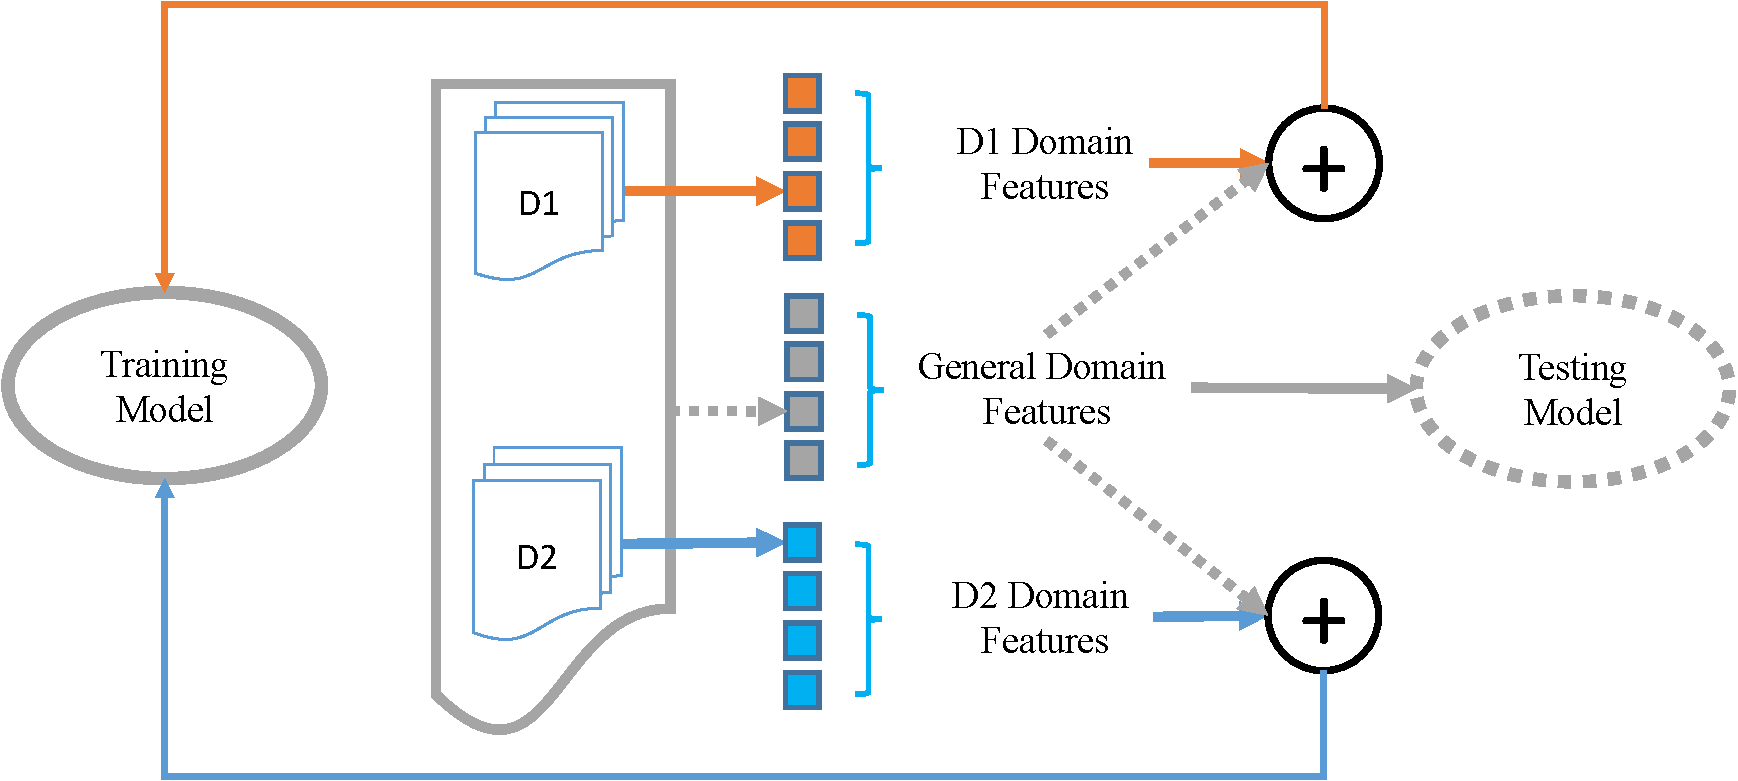
\includegraphics[width=0.60\textwidth]{images/chapter2/feature-aug.pdf}
\caption{Illustration of Frustratingly Easy Domain Adaptation~\cite{daume2007frustratingly}. We present a collection of documents that are from two different domains, ``D1'' and ``D2''. Three different colors of features means domain-specific (blue and orange) and domain-independent (or called general, gray) features. For the test step, domain features are optional, instead, we can just use the domain-independent features.}
\label{chap2:fig:aug}
\end{figure}

Feature augmentation in domain adaptation aims to obtain domain independent representation of documents and therefore generalize document classifiers~\cite{blitzer2006domain, daume2007frustratingly}.
We show a feature augmentation method in Figure~\ref{chap2:fig:aug}.
The methods show its effectiveness in user factor~\cite{lynn2017human} and temporality~\cite{huang2018examining} adaptation for improving and generalizing document classifiers.
The method first extracts features within each domain, domain specific features.
Next, by treating all documents as a whole, the methods extract general features, domain-independent features.
We can format a document representation by a combination of domain specific and independent features: $\langle X_g, X_{d1}, X_{d2} \rangle$.
A document from ``D1'' domain can be represented as $\langle X_g, X_{d1}, 0 \rangle$, and similarly, a document from ``D2'' domain can be represented as $\langle X_g, 0, X_{d2} \rangle$. 
After feeding the features to document classifiers, 
we can optimize a domain-independent document classifier, which can generalize better across all domains.
During the test, if the domain of test documents is known, we can feed the combined features to the classifier, if not known, we can just feed the general features to the trained document classifiers.


\subsection{Multitask Learning}

\begin{figure}[tb!]
\centering
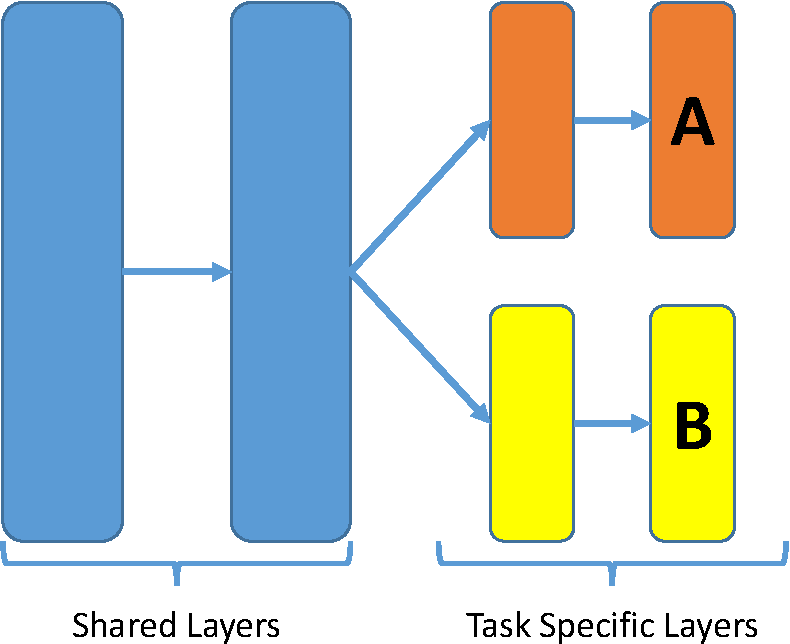
\includegraphics[width=0.45\textwidth]{images/chapter2/multitask.pdf}
\caption{Illustration of Multitask Learning with the neural model. This MTL architecture contains shared and task specific layers. The A and B can be different prediction tasks.}
\label{chap2:fig:mtl}
\end{figure}

The Figure~\ref{chap2:fig:mtl} presents a Multitask Learning (MTL) framework with a neural model architecture.
The model shares two tasks with the same first few layers while leaves task specific layers for each task.
The MTL improves and generalizes each prediction task from the following three main aspects.
First, adding one more prediction task can bring more training instances for tweaking the shared layers. 
Second, the prediction tasks force the model learning task independent representations and improve generalization by leveraging the domain-specific information contained in the training signals of related tasks~\cite{Caruana1997multitask}.
Third, the task specific layers can help learn task specific patterns for document classifiers.

% http://ruder.io/multi-task/

\subsection{Domain Adversarial Training}

Domain adversarial training is a method to enable document representations less sensitive and predictable towards domain categories so that models can generalize across domains~\cite{ganin2016domain}.
The method assumes there are two domains, source and target domains, where source domain documents have labels and target domain documents do not.
There are two main loss function based on the categorical cross entropy function~\cite{goodfellow2016deep}: document class and domain predictions.
The domain class prediction is the regular prediction task, while the domain prediction is to predict if a document belongs to the source or target domain.
To generalize the document representations, the method aims to penalize high accuracy of domain prediction.
Therefore, the method reverse the loss value of domain prediction, we can then have the following:
$$Loss = \frac{1}{n}\sum_{i=1}^n\mathcal{L}(y_i, \hat{y}_i) - \lambda(\frac{1}{n}\sum_{i=1}^n\mathcal{L}(y_s, \hat{y}_d) + \frac{1}{\hat{n}}\sum_{i=n+1}^N\mathcal{L}(y_t, \hat{y}_d))$$
, where $N$ is the total number of documents from both source and target domains, $n$ is the number of labeled documents from the source domain, $\hat{n}$ is the number of unlabeled documents from the target domain, $y$ refers to document label and $\hat{y}$ is the predicted document class, $\lambda$ indicates the weight of document prediction loss, $y_s$ and $y_t$ are the domain labels for source and target respectively, and $\hat{y}_d$ refers to the predicted domain label.
Noted that usually, the final loss values are sum of all loss functions.
However, the domain adversarial training reverse the plus to minus in the function above, which can be viewed as an ``adversarial'' way.
And the adversarial optimization only happens during the training step.
Therefore, the method is called ``domain adversarial training''. 


\section{Temporal Variations of Language}
\label{chap2:sec:time}

\begin{figure}[tb!]
\centering
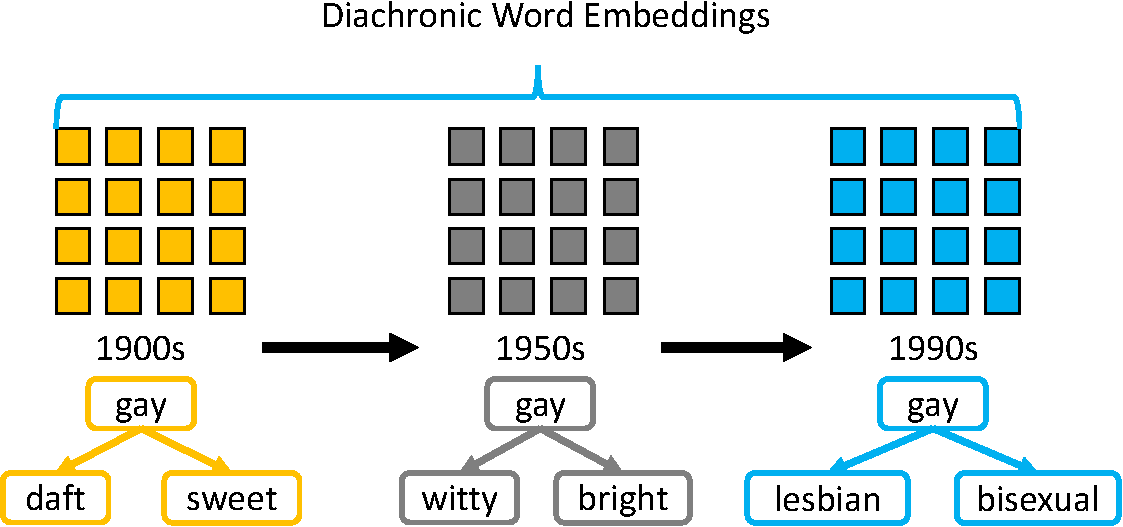
\includegraphics[width=0.55\textwidth]{images/chapter2/diachronic.pdf}
\caption{Illustration of Diachronic Word Embeddings. We introduce an existing method~\cite{kulkarni2015statistically} to train diachronic word embeddings. The three time intervals use different colors to distinguish embedding models and dynamics of temporal semantics. With the selected three time intervals (1900s, 1950s, 1990s) and diachronic word embeddings, we present a case study that how the word ``gay'' changes its close synonyms over time.}
\label{chap2:fig:diachronic}
\end{figure}

\subsection{Language Shifts}

Language, and therefore data derived from language, changes over time~\cite{Ullmann62}.
\textit{Language shift} reflects the complex mutual processes between language and human society overtime.
Word senses can shift over long periods of time \cite{hamilton2016diachronic}, and written language can change rapidly in online platforms \cite{eisenstein2014diffusion, goel2016social}.
For example, the meaning of \textit{gay} has changed from \textit{cheerful} to \textit{homosexual}~\cite{hamilton2016diachronic}, and the emoji have only become available in recent years. 

Time is implicitly embedded in the classification process: classifiers are often built to be applied to future data that doesn't yet exist, and performance on held-out data is measured to estimate performance on future data whose distribution may have changed.
One promising solution is \textit{diachronic word embedding}, which jointly models words and temporality.


\subsection{Diachronic Word Embedding}

Diachronic word embedding\footnote{Also called dynamic word embeddings~\cite{yao2018dynamic}.} (DWE) explicitly models temporality into word embedding models to capture the change of word semantic meaning~\cite{kutuzov2018diachronic}.
Existing research utilizes the diachronic word embedding into different tasks under the topic of semantic shifts~\cite{kutuzov2018diachronic}, such as semantic shift detection~\cite{mihalcea2012word, kim2014temporal, kulkarni2015statistically, rudolph2018dynamic, yao2018dynamic, rosenfeld2018deep}, laws of semantic change~\cite{hamilton2016diachronic, dubossarsky2017outta}, diachronic semantic relations~\cite{rosin2017learning, szymanski2017temporal}, etc.

The Figure~\ref{chap2:fig:diachronic} illustrates an example of building diachronic word embedding.
First a corpus will be split into different time intervals, which can be seasonal~\cite{huang2018examining}, yearly~\cite{yao2018dynamic}, decade~\cite{hamilton2016diachronic}:
$$C = [d_{1, 1}, ~d_{2, 1}, ~..., ~d_{i, t}] $$
$$C_t \in C, ~~~ C_t = [d_{1, t},~ ...d_{n, t}]$$
, where $C$ is the corpus, $d$ is a document, $i$ is the index of document and $t$ is the time label, $C_t$ is a collection of documents within the $t$ time interval and $n$ is the number of documents in $C_t$.
Next, a word embedding model for each time interval will be trained for each time interval.
However, due to training the embedding models separately for each time interval causes the unaligned vector spaces, our next step is to map the embedding models into the same vector space:
$$f(W, E_{\hat{t}}) = E_t$$
, where $\hat{t}$ and $t$ are source and target time intervals respectively, $E$ is an embedding model, $f$ is the alignment function and $W$ is the function weight to learn.

Existing methods of aligning word embeddings focus on the following three directions: incremental training~\cite{kim2014temporal}, matrix transformation~\cite{kulkarni2015statistically, hamilton2016diachronic, yao2018dynamic} and integrated vectors of time and word~\cite{rosenfeld2018deep, huang2019neural}. \textit{Incremental Training} utilizes the trained embedding model to initialize the embedding weights of words in the next time interval.
\textit{Matrix Transformation} learns a transformation matrix $M \in R^{d \times d}$ by solving the following optimization:
$$argmin \sum_{i=1}^{|V|}|E_t(w_i) - E_{\hat{t}} \cdot M|^2$$
, where $|V|$ is the vocabulary size, $w_i$ is a word from the vocabulary.
\textit{Integrated vectors of time and word} model time label and word jointly. In contrast to the regular word representations, the new representation with both time and word will be:
$$\hat{E}(w_i) = f(E(w_i) \cdot W_w + T_e(t) \cdot W_t)$$
, where $\hat{E}$ is the new word embedding, $T_e$ is an embedding model of time labels, $w_i$ is a word, $f$ is an activation function to model word and time jointly, $W$ is the weight.
Training the model is similar to word embeddings in Section~\ref{chap2:subsubsec:emb}, except the $U$ and $W$ will incorporate both time and word vectors.


\subsubsection{DWE Evaluation}

Existing DWE evaluation methods~\cite{kutuzov2018diachronic} fall into three prediction tasks: cross-time analogy, time span disambiguation and event prediction.
\textit{Cross-time analogy}~\cite{szymanski2017temporal, yao2018dynamic} is to find semantic equivalents across time intervals.
For example, US president is close to Obama in 2015 vs. Trump in 2017 and Apple is close to fruit in 1980 vs. Microsoft in 2018.
\textit{Time span disambiguation}~\cite{mihalcea2012word, popescu2015semeval} is to determine the specific time spans that documents or words belong to. 
For example, diachronic text evaluation~\cite{popescu2015semeval} split documents into different time intervals and evaluate if classifiers can predict correctly the time intervals of documents.
\textit{Event prediction}~\cite{kutuzov2017tracing} is to use diachronic word embeddings to predict or trace real-world events such as gun violations and conflicts.


\section{Demographic Variations of Language}
\label{chap2:sec:demographic}

% \paragraph{Demographic prediction} is a common task in natural language processing.
Language varies across demographic factors. 
Research has shown that social media text is predictive of demographic variables such as 
gender~\cite{Rao:2010:CLU:1871985.1871993,Rao2011,Burger:2011:DGT:2145432.2145568,volkova2015inferring}, age~\cite{rosenthal2011age, hovy2015tagging,johannsen2015cross, zhang2016predicting, diaz2018addressing}, race~\cite{preoctiuc2018user} and location~\cite{EisensteinEtAl10,wing2011simple,wing2014hierarchical}.
For example, male and female express sentiment differently and young people use more widely emoji in their social media than elders.
Such variations can also cause biases of document classifiers towards a specific demographic group~\cite{sun2019mitigating}.
Research show that hate speech classifiers tend to classify African American English words as hate crime, yet such words might strongly correlate with the specific racial group and cause racial biases~\cite{davidson2019racial, sap2019risk}.
Therefore, it is necessary to model the user demographic factors into document classifiers.


\subsection{User Factor Adaptation}

\textit{User factor adaptation} integrates user demographic factors and histories into the machine learning classifiers. The demographic factors usually refer to the attributes of users, such as gender, age, geographic location, etc. Online generated user texts show demographic variations in the linguistic styles, and the linguistic style differences could be used for the use factor prediction~\cite{rosenthal2011age, zhang2016predicting, hovy2018improving}. The user histories are the historical contexts of users, such as previous posts or likes or retweets of the users. The user factors impact on how online users express their opinions and show promising improvements in the text classification task~\cite{volkova2013exploring, hovy2015demographic, lynn2017human, yang2017overcoming}.

Lynn et al~\cite{lynn2017human} use a feature augmentation method~\cite{daume2007frustratingly} to adapt user factors into document classifiers.
The method extract two types of features: general and user attribute dependent features. 
For example, assuming that we have a document, the user age attribute and we split the age into two categories, $>24 or \leq 24$.
Then the method can represent the document with the author age 20 as:
$$<X_g, X_{a\leq24}, 0>$$
, where $X_g$ is the general feature set, and $X_a$ is the age dependent feature set.
Alternatively, a document with the author age 30 as:
$$<X_g, 0, X_{a>24}>$$
Finally, the method can train a document classifier with the augmented feature sets.
For the theoretical details, please refer to Section~\ref{chap2:subsec:feaaug}.

\subsubsection{User Embeddings}

\begin{figure}[tb!]
\centering
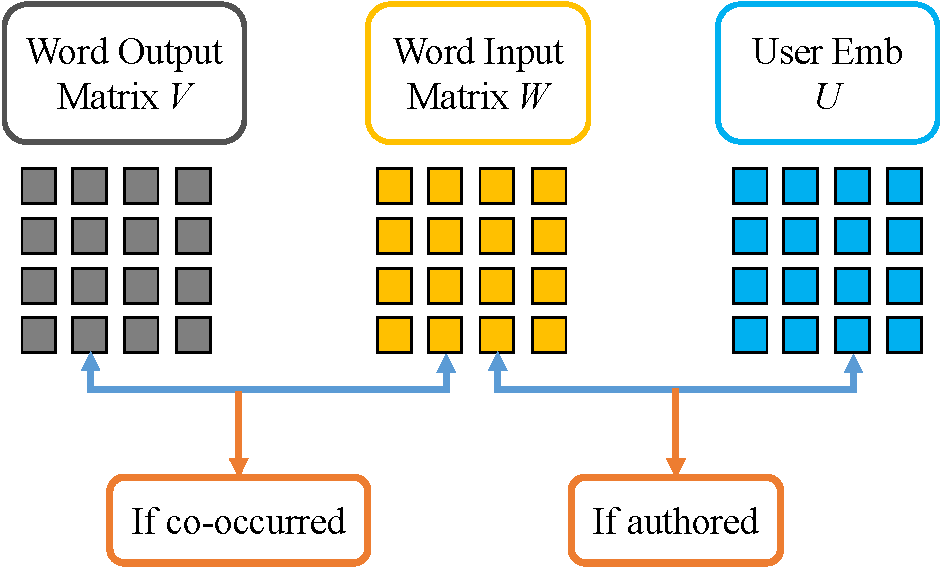
\includegraphics[width=0.55\textwidth]{images/chapter2/user-emb.pdf}
\caption{Illustration of Training User Embeddings via Skip-gram~\cite{amir2017quantifying}. $V$ is the randomly initialized output matrix of word representations, $W$ is the randomly initialized input matrix of word representations, and $U$ is the randomly initialized matrix of user embedding.}
\label{chap2:fig:user}
\end{figure}

User embedding is to model latent human traits and behaviors and map the features into a fixed low dimensional representations~\cite{pan2019social}. 
Common features include user generated reviews, user profiles and networking connections. 
Yet, not every dataset have the networking connections, this thesis only consider user generated text documents and profile information.
To generate the user features, researchers have proposed various approaches including n-gram features~\cite{benton2016learning}, LDA~\cite{zhang2015using, ding2017multi}, Word2vec~\cite{amir2016modelling, benton2016learning, amir2017quantifying, wu2018starspace}, Doc2vec~\cite{ding2017multi, ding2018predicting}, etc.
The generated user features are usually multiple views of user behaviors. 
To map the multi-view features into a fixed representation, researchers have deployed methods including concatenation~\cite{pennacchiotti2011a}, average~\cite{ding2017multi}, Generalized Canonical Correlation Analysis (GCCA)~\cite{benton2016learning}.

% skip-gram~\cite{amir2016modelling}
Using Skip-gram to jointly train word and user embeddings is a common way to obtain fixed representations of users~\cite{amir2017quantifying, wu2018starspace}, as shown in Figure~\ref{chap2:fig:user}.
The model jointly trains two prediction tasks at the same time: predicting if the input words are mutual contexts or not and if users used the input words.


\subsection{Fairness in NLP}

\textit{Demographic bias} has been shown to be encoded in machine learning models. 
Fairness is especially critical to the public health research, which analyzes across demographic groups over time. 
Language variations across the demographic factors have raised people's concerns that the demographic variations can prohibit building \textit{fair} document classifiers~\cite{sun2019mitigating, bender2018data}. 
For example, unintended bias~\cite{dixon2018measuring}, which highly correlates with the demographic factors, will make classifiers discriminatory in that classifiers will perform better for some demographic groups than others. 
Word embeddings, which are widely used in classification tasks, are prone to learning demographic stereotypes.
For example, a study~\cite{bolukbasi2016man} found that the word ``programmer'' is more similar to ``man'' than ``woman'', while ``receptionist'' is more similar to ``woman''.

\subsubsection{Debiasing Methods}

To reduce learning biases for document classifiers, existing research fall into three main directions: debiased word embeddings~\cite{zhao2017men}, data augmentation~\cite{dixon2018measuring, zhao2019gender} and model fine tuning~\cite{park2018reducing}.
\textit{Debiased Word Embeddings} is to adjust embeddings the distance balance between demographic related pronouns and concepts, such as he/she with engineer.
\textit{Data Augmentation} is to neutralize document classifiers by changing training corpora: word blindness or replacement. 
The core idea is to either remove demographic pronouns or replace sensitive words with neutralized words.
For example, we can remove gender related words including  ``he/she'' or ``male/female'' from the corpora to prevent classifiers judging the documents by the sensitive words.
\textit{Model Fine Tuning} focuses on adjusting trained models on the target dataset. The method first trained a document classifier on a larger and less-biased corpus, which is similar to the target corpus. 
Next, the method adjusts hyperparameters of the trained model based on the target corpus, which is smaller and more biased than the source data.


\subsubsection{Fairness Evaluation}

Bias and fairness of document classifiers focus on examining how document classifiers perform differently across demographic groups, such as male and female.
In this thesis proposal, we particularly focus on group fairness measurement~\cite{hardt2016equality}. 
The motivation is to evaluate equal opportunity between demographic groups.
Existing research~\cite{dixon2018measuring, garg2019counterfactual, park2018reducing} evaluate the author-level fairness of document classifiers by: AUC and \textit{equality differences} (ED) of true positive/negative and false positive/negative rates.

The ED sums the differences between the rates within specific user groups and the overall rates:
$$ED = \sum_{g \in G}|Rate - Rate_g|$$
, where the G is a demographic group, g is one type in the group, $Rate$ indicates one of true positive/negative and false positive/negative rates across the whole group, and $Rate_g$ is a rate of a type such as female's false positive rate.